\ofsection{FFRPG 4e rules}
%
The following is a collection of optional rules and content for the Final Fantasy Role Playing Game 4th Edition~ \textbf{(FFRPG 4e)}, which you can use to create a closer feeling to Final Fantasy Tactics.
%
\\\\
%
\ofaccent{\large Optional Map Combat Rules} \ofrow
Groups willing to experience an even more detailed combat system may use this optional mode for some or even all of its combat encounters. 
Use this optional system to simulate the strategy elements of the original Final Fantasy Tactics game. 
Be wary, however, that this implies a genre change and will place even more focus on the combat aspect of the game.
%
\ofrow
%
\ofaccent{The MOVE stat:} Add the \textbf{MOVE} stat for each character. 
It means the total number of squares the character may move with the \textbf{!Move} action. 
All characters start with a MOVE stat of 4, increasing by 1 for each 6 levels of the Air stat. Abilities and Statuses may affect the MOVE stat.\\
\ofaccent{Weaken (Speed):} Move reduced by 1.\\
\ofaccent{Strengthen (Speed):} Move increased by 1.\\
\ofaccent{Toad:} Move reduced to 1.\\
\ofaccent{Berserk:} The character will move as close as possible to the nearest target within their line of sight before attacking, if able.\\
\ofaccent{Confuse:} Roll for confuse as normal; randomly pick a target that is within reach in accordance with the confuse roll. 
If this is not possible, decide radomly a cardinal direction, and then move as far as possible in that direction.\\
\ofaccent{Float:} The character is less hampered by harsh terrain.\\
\ofaccent{Flying:} Ignore all terrain while moving.\\
\ofaccent{Immobilize:} Move reduced to zero.\\
\ofaccent{Stone:} The character, as implied by the text, cannot move or act.\\
\ofaccent{Sleep:} The character, as implied by the text, cannot move or act.\\
\ofaccent{Stop:} The character, as implied by the text, cannot move or act.
%
\\\\
%
\ofaccent{New Basic Action - !Move:} All characters gain the \textbf{!Move} action.
You may use an action to move a number of squares up to your MOVE stat. 
Once per round, when doing any action (but not during a reaction) you may also use the \textbf{!Move} action as a free action. 
If you do so, you can move either before or after doing the action. 
When moving, you walk in orthogonal directions counting one square at a time, so to move in a diagonal path you must spend two squares of movement for each diagonal square you walk (one forward then one to the left/right).
If the target of an ability moves during the windup of a Slow action, the ability remains targeted on them, as long as they remain within range. 
If a target moves outside the range of a Slow action, the character acting may retarget his action to another valid target in range.
A character charging a Slow action can do a \textbf{!Move} action (either as a free action or by using an interrupt or delayed action), and move at the start of the phase before the Slow action is executed.
A character or monster may freely move through any allied space as long as they do not stop in the same space as their ally. 
They cannot move through a square occupied by a foe. 
Whenever you do a successful \textbf{!Flee} action, you may also move a number of squares equal to your Move stat.
%
\\\\
%
\ofaccent{Zone of Control:} Characters wielding Melee weapons, or that can do Melee attacks for any reason (for example, an Archer who has the Point-Blank Specialty wielding a ranged weapon) project Zone of Control.
Your Zone of Control is equal to all squares you can hit with a melee attack. 
Any enemy who tries to leave your \textbf{Zone of Control} must be successful with a \textbf{!Flee} action to do so.
Moving into a Zone of Control or any movement that does not leave a character's Zone of Control is unimpeded.
Forced movement (for example, if someone pushes or pulls a character) also ignores Zone of Control. 
Unarmed attacks do not project Zone of Control, as does any character with a status effect that prevents him from doing actions (\textbf{Sleep}, \textbf{Stop}, \textbf{Stone} and \textbf{Disable}). 
Reduce by 25 the difficulty of using \textbf{!Flee} against a target with the Blind status effect.
%
\\\\
%
\ofaccent{Weapon Range:} Some weapons are able to attack from further away than others. 
The \textbf{Range} is the number of spaces away from the character that they may attack. 
All weapons will also follow a Line of Effect, so should an obstacle or another target be in-between the Character and their chosen target, the attack will instead hit the first obstacle or target in the Line of Effect.\ofrow 
\ofaccent{Light Swords/Knives, Weapons \& Shield, Heavy Weapons, Claws/Gloves, Staves, Twin Blades:} Any square adjacent or directly diagonal to the attacker.\ofrow
\ofaccent{Polearms:} Any square up to 2 squares from the attacker.\ofrow
\ofaccent{Throwing Weapons, Wands, Instruments:} Any square up to four squares from the attacker.\ofrow
\ofaccent{Bows, Rifles/Crossbows:} Any square up to five squares from the attacker. \ofrow
\ofaccent{Shotgun:} Cone: 3.
%
\\\\
%
\ofaccent{Other Ranges:} All other ranges are written using the following notation: "R: Number; E: Number".
R means range and “Number” is the number of squares away from the user where the user can select the target. 
An R rating of zero means the origin square of the effect is the user. 
E means effect and “Number” is the width of the effect, in squares. 
An E rating of zero means the effect targets only one square. 
For other range or effect ratings, see the diagrams below.
The blue square means the origin (either the character for the origin of the Range or the origin square for the origin of
the Effect), while the red squares mean either the squares that may be selected as the origin square (Range) or the squares affected by it (Effect). For Cones and Bursts, the origin square is not under the effects of the spell/ability, unless the ability or spell says otherwise.
%
\\\\
%
\ofaccent{Normal Ranges or Areas: RN or EN}
\begin{figure}[h!]
	\centering
	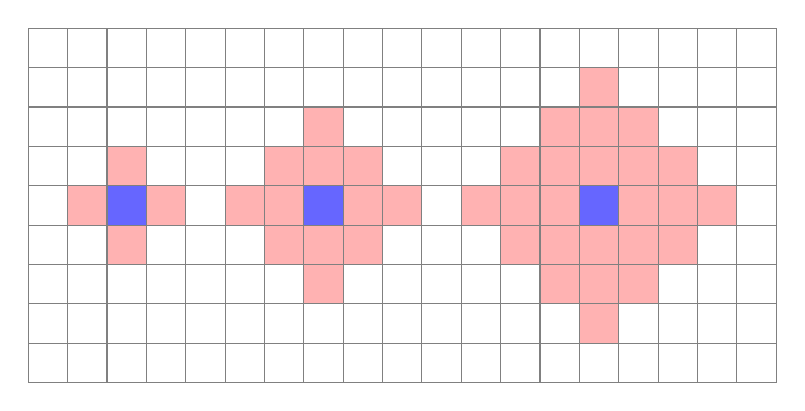
\begin{tikzpicture}[]
	\tikzstyle{filled}=[draw, black!50!white, rectangle, thin, minimum height = 0.5cm, minimum width=0.5cm]
	\tikzstyle{target}=[fill=red!30!white]
	\tikzstyle{caster}=[fill=blue!60!white]
	\tikzstyle{obstacle}=[fill=black!100!white]	
	\draw[step=0.5,black!50!white, thin,xshift=-0.25cm,yshift=-0.25cm] (0,0) grid (9.5, 4.5);	
	%E:1 
		%Center
	\node[filled, caster](g0)at (1.0, 2.0) {};
		%First Ring
	\node[filled, target](g0)at (1.0, 1.5) {};
	\node[filled, target](g0)at (1.5, 2.0) {};
	\node[filled, target](g0)at (1.0, 2.5) {};
	\node[filled, target](g0)at (0.5, 2.0) {};
	%E:2
		%Center
	\node[filled, caster](g0)at (3.5, 2.0) {};
		%First Ring
	\node[filled, target](g0)at (3.5, 1.5) {};
	\node[filled, target](g0)at (4.0, 2.0) {};
	\node[filled, target](g0)at (3.5, 2.5) {};
	\node[filled, target](g0)at (3.0, 2.0) {};
		%Second Ring
	\node[filled, target](g0)at (3.5, 1.0) {};
	\node[filled, target](g0)at (3.0, 1.5) {};
	\node[filled, target](g0)at (2.5, 2.0) {};
	\node[filled, target](g0)at (3.0, 2.5) {};
	\node[filled, target](g0)at (3.5, 3.0) {};
	\node[filled, target](g0)at (4.0, 2.5) {};
	\node[filled, target](g0)at (4.5, 2.0) {};
	\node[filled, target](g0)at (4.0, 1.5) {};
	%E:3
		%Center
	\node[filled, caster](g0)at (7.0, 2.0) {};
		%First Ring
	\node[filled, target](g0)at (7.0, 1.5) {};
	\node[filled, target](g0)at (7.5, 2.0) {};
	\node[filled, target](g0)at (7.0, 2.5) {};
	\node[filled, target](g0)at (6.5, 2.0) {};
		%Second Ring
	\node[filled, target](g0)at (7.0, 1.0) {};
	\node[filled, target](g0)at (6.5, 1.5) {};
	\node[filled, target](g0)at (6.0, 2.0) {};
	\node[filled, target](g0)at (6.5, 2.5) {};
	\node[filled, target](g0)at (7.0, 3.0) {};
	\node[filled, target](g0)at (7.5, 2.5) {};
	\node[filled, target](g0)at (8.0, 2.0) {};
	\node[filled, target](g0)at (7.5, 1.5) {};
		%Third Ring
	\node[filled, target](g0)at (7.0, 0.5) {};
	\node[filled, target](g0)at (7.5, 1.0) {};
	\node[filled, target](g0)at (8.0, 1.5) {};
	\node[filled, target](g0)at (8.5, 2.0) {};
	\node[filled, target](g0)at (8.0, 2.5) {};
	\node[filled, target](g0)at (7.5, 3.0) {};
	\node[filled, target](g0)at (7.0, 3.5) {};
	\node[filled, target](g0)at (6.5, 3.0) {};
	\node[filled, target](g0)at (6.0, 2.5) {};
	\node[filled, target](g0)at (5.5, 2.0) {};
	\node[filled, target](g0)at (6.0, 1.5) {};
	\node[filled, target](g0)at (6.5, 1.0) {};

\end{tikzpicture}
\end{figure}

\ofaccent{Orthogonal Ranges or Areas: RN\# or EN\#} 
\begin{figure}[h!]
	\centering
	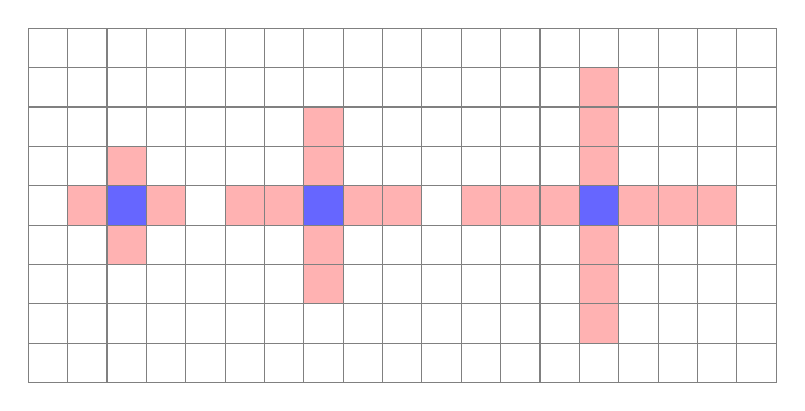
\begin{tikzpicture}[]
	\tikzstyle{filled}=[draw, black!50!white, rectangle, thin, minimum height = 0.5cm, minimum width=0.5cm]
	\tikzstyle{target}=[fill=red!30!white]
	\tikzstyle{caster}=[fill=blue!60!white]
	\tikzstyle{obstacle}=[fill=black!100!white]	
	\draw[step=0.5,black!50!white, thin,xshift=-0.25cm,yshift=-0.25cm] (0,0) grid (9.5, 4.5);	
	%E:1 
		%Center
	\node[filled, caster](g0)at (1.0, 2.0) {};
		%First Ring
	\node[filled, target](g0)at (1.0, 1.5) {};
	\node[filled, target](g0)at (1.5, 2.0) {};
	\node[filled, target](g0)at (1.0, 2.5) {};
	\node[filled, target](g0)at (0.5, 2.0) {};
	%E:2
		%Center
	\node[filled, caster](g0)at (3.5, 2.0) {};
		%First Ring
	\node[filled, target](g0)at (3.5, 1.5) {};
	\node[filled, target](g0)at (4.0, 2.0) {};
	\node[filled, target](g0)at (3.5, 2.5) {};
	\node[filled, target](g0)at (3.0, 2.0) {};
		%Second Ring
	\node[filled, target](g0)at (3.5, 1.0) {};
	\node[filled, target](g0)at (2.5, 2.0) {};
	\node[filled, target](g0)at (3.5, 3.0) {};
	\node[filled, target](g0)at (4.5, 2.0) {};
	%E:3
		%Center
	\node[filled, caster](g0)at (7.0, 2.0) {};
		%First Ring
	\node[filled, target](g0)at (7.0, 1.5) {};
	\node[filled, target](g0)at (7.5, 2.0) {};
	\node[filled, target](g0)at (7.0, 2.5) {};
	\node[filled, target](g0)at (6.5, 2.0) {};
		%Second Ring
	\node[filled, target](g0)at (7.0, 1.0) {};
	\node[filled, target](g0)at (6.0, 2.0) {};
	\node[filled, target](g0)at (7.0, 3.0) {};
	\node[filled, target](g0)at (8.0, 2.0) {};
		%Third Ring
	\node[filled, target](g0)at (7.0, 0.5) {};
	\node[filled, target](g0)at (8.5, 2.0) {};
	\node[filled, target](g0)at (7.0, 3.5) {};
	\node[filled, target](g0)at (5.5, 2.0) {};

\end{tikzpicture}
\end{figure}

\ofaccent{Cone: Cone N}
\begin{figure}[h!]
	\centering
	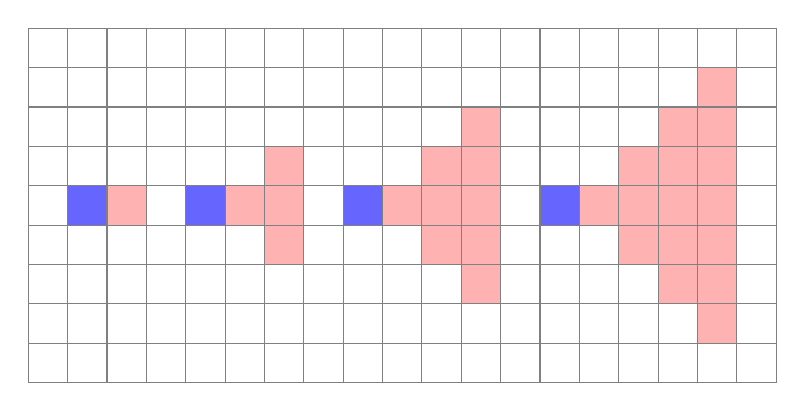
\begin{tikzpicture}[]
	\tikzstyle{filled}=[draw, black!50!white, rectangle, thin, minimum height = 0.5cm, minimum width=0.5cm]
	\tikzstyle{target}=[fill=red!30!white]
	\tikzstyle{caster}=[fill=blue!60!white]
	\tikzstyle{obstacle}=[fill=black!100!white]	
	\draw[step=0.5,black!50!white, thin,xshift=-0.25cm,yshift=-0.25cm] (0.5,0) grid (10, 4.5);	
	%E:1 
		%Center
	\node[filled, caster](g0)at (1.0, 2.0) {};
		%First Ring
	\node[filled, target](g0)at (1.5, 2.0) {};
	%E:2
		%Center
	\node[filled, caster](g0)at (2.5, 2.0) {};
		%First Ring
	\node[filled, target](g0)at (3.0, 2.0) {};
		%Second Ring
	\node[filled, target](g0)at (3.5, 1.5) {};
	\node[filled, target](g0)at (3.5, 2.0) {};
	\node[filled, target](g0)at (3.5, 2.5) {};
	%E:3
		%Center
	\node[filled, caster](g0)at (4.5, 2.0) {};
		%First Ring
	\node[filled, target](g0)at (5.0, 2.0) {};
		%Second Ring
	\node[filled, target](g0)at (5.5, 1.5) {};
	\node[filled, target](g0)at (5.5, 2.0) {};
	\node[filled, target](g0)at (5.5, 2.5) {};
		%Third Ring
	\node[filled, target](g0)at (6.0, 1.0) {};
	\node[filled, target](g0)at (6.0, 1.5) {};
	\node[filled, target](g0)at (6.0, 2.0) {};
	\node[filled, target](g0)at (6.0, 2.5) {};
	\node[filled, target](g0)at (6.0, 3.0) {};
		%E:4
	%Center
	\node[filled, caster](g0)at (7.0, 2.0) {};
		%First Ring
	\node[filled, target](g0)at (7.5, 2.0) {};
		%Second Ring
	\node[filled, target](g0)at (8.0, 1.5) {};
	\node[filled, target](g0)at (8.0, 2.0) {};
	\node[filled, target](g0)at (8.0, 2.5) {};
		%Third Ring
	\node[filled, target](g0)at (8.5, 1.0) {};
	\node[filled, target](g0)at (8.5, 1.5) {};
	\node[filled, target](g0)at (8.5, 2.0) {};
	\node[filled, target](g0)at (8.5, 2.5) {};
	\node[filled, target](g0)at (8.5, 3.0) {};
		%Fourth Ring
	\node[filled, target](g0)at (9.0, 0.5) {};
	\node[filled, target](g0)at (9.0, 1.0) {};
	\node[filled, target](g0)at (9.0, 1.5) {};
	\node[filled, target](g0)at (9.0, 2.0) {};
	\node[filled, target](g0)at (9.0, 2.5) {};
	\node[filled, target](g0)at (9.0, 3.0) {};
	\node[filled, target](g0)at (9.0, 3.5) {};
		
\end{tikzpicture}
\end{figure}

\ofaccent{Burst: Burst N}
\begin{figure}[h!]
	\centering
	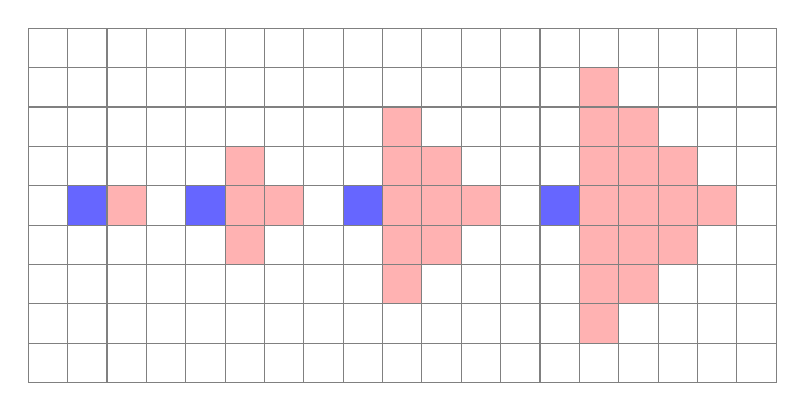
\begin{tikzpicture}[]
	\tikzstyle{filled}=[draw, black!50!white, rectangle, thin, minimum height = 0.5cm, minimum width=0.5cm]
	\tikzstyle{target}=[fill=red!30!white]
	\tikzstyle{caster}=[fill=blue!60!white]
	\tikzstyle{obstacle}=[fill=black!100!white]	
	\draw[step=0.5,black!50!white, thin,xshift=-0.25cm,yshift=-0.25cm] (0.5,0) grid (10, 4.5);	
	%E:1 
		%Center
	\node[filled, caster](g0)at (1.0, 2.0) {};
		%First Ring
	\node[filled, target](g0)at (1.5, 2.0) {};
	%E:2
		%Center
	\node[filled, caster](g0)at (2.5, 2.0) {};
		%First Ring
	\node[filled, target](g0)at (3.0, 1.5) {};
	\node[filled, target](g0)at (3.0, 2.0) {};
	\node[filled, target](g0)at (3.0, 2.5) {};
		%Second Ring
	\node[filled, target](g0)at (3.5, 2.0) {};
	%E:3
		%Center
	\node[filled, caster](g0)at (4.5, 2.0) {};
		%First Ring
	\node[filled, target](g0)at (5.0, 1.0) {};
	\node[filled, target](g0)at (5.0, 1.5) {};
	\node[filled, target](g0)at (5.0, 2.0) {};
	\node[filled, target](g0)at (5.0, 2.5) {};
	\node[filled, target](g0)at (5.0, 3.0) {};
		%Second Ring
	\node[filled, target](g0)at (5.5, 1.5) {};
	\node[filled, target](g0)at (5.5, 2.0) {};
	\node[filled, target](g0)at (5.5, 2.5) {};
		%Third Ring
	\node[filled, target](g0)at (6.0, 2.0) {};
		%E:4
	%Center
	\node[filled, caster](g0)at (7.0, 2.0) {};
		%First Ring
	\node[filled, target](g0)at (7.5, 0.5) {};
	\node[filled, target](g0)at (7.5, 1.0) {};
	\node[filled, target](g0)at (7.5, 1.5) {};
	\node[filled, target](g0)at (7.5, 2.0) {};
	\node[filled, target](g0)at (7.5, 2.5) {};
	\node[filled, target](g0)at (7.5, 3.0) {};
	\node[filled, target](g0)at (7.5, 3.5) {};
		%Second Ring
	\node[filled, target](g0)at (8.0, 1.0) {};
	\node[filled, target](g0)at (8.0, 1.5) {};
	\node[filled, target](g0)at (8.0, 2.0) {};
	\node[filled, target](g0)at (8.0, 2.5) {};
	\node[filled, target](g0)at (8.0, 3.0) {};
		%Third Ring
	\node[filled, target](g0)at (8.5, 1.5) {};
	\node[filled, target](g0)at (8.5, 2.0) {};
	\node[filled, target](g0)at (8.5, 2.5) {};
		%Fourth Ring
	\node[filled, target](g0)at (9.0, 2.0) {};
\end{tikzpicture}
\end{figure}
%
\pagebreak\\
%
\ofaccent{Line: Line N and Adjacent Diagonals: E1*} 
\begin{figure}[h!]
	\centering
	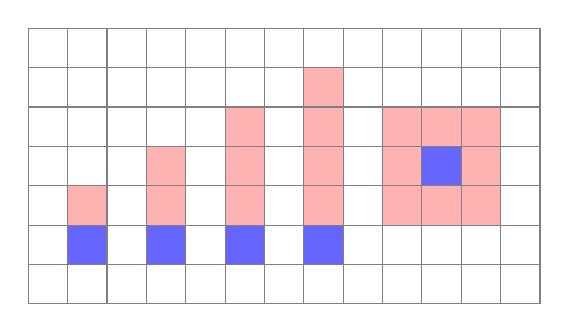
\begin{tikzpicture}[]
	\tikzstyle{filled}=[draw, black!50!white, rectangle, thin, minimum height = 0.5cm, minimum width=0.5cm]
	\tikzstyle{target}=[fill=red!30!white]
	\tikzstyle{caster}=[fill=blue!60!white]
	\tikzstyle{obstacle}=[fill=black!100!white]	
	\draw[step=0.5,black!50!white, thin,xshift=-0.25cm,yshift=-0.25cm] (0,0) grid (6.5, 3.5);	
	%E:1 
		%Center
	\node[filled, caster](g0)at (0.5, 0.5) {};
		%First Ring
	\node[filled, target](g0)at (0.5, 1.0) {};
	%E:2
		%Center
	\node[filled, caster](g0)at (1.5, 0.5) {};
		%First Ring
	\node[filled, target](g0)at (1.5, 1.0) {};
		%Second Ring
	\node[filled, target](g0)at (1.5, 1.5) {};
	%E:3
		%Center
	\node[filled, caster](g0)at (2.5, 0.5) {};
		%First Ring
	\node[filled, target](g0)at (2.5, 1.0) {};
		%Second Ring
	\node[filled, target](g0)at (2.5, 1.5) {};
		%Third Ring
	\node[filled, target](g0)at (2.5, 2.0) {};
	%E:4
		%Center
	\node[filled, caster](g0)at (3.5, 0.5) {};
		%First Ring
	\node[filled, target](g0)at (3.5, 1.0) {};
		%Second Ring
	\node[filled, target](g0)at (3.5, 1.5) {};
		%Third Ring
	\node[filled, target](g0)at (3.5, 2.0) {};
		%Fourth Ring
	\node[filled, target](g0)at (3.5, 2.5) {};
	%E1*
		%Center
	\node[filled, caster](g0)at (5.0, 1.5) {};
		%First Ring
	\node[filled, target](g0)at (5.5, 1.0) {};
	\node[filled, target](g0)at (5.0, 1.0) {};
	\node[filled, target](g0)at (4.5, 1.0) {};
	\node[filled, target](g0)at (5.0, 2.0) {};
	\node[filled, target](g0)at (5.5, 2.0) {};
	\node[filled, target](g0)at (4.5, 2.0) {};
	\node[filled, target](g0)at (5.5, 1.5) {};
	\node[filled, target](g0)at (4.5, 1.5) {};
\end{tikzpicture}
\end{figure}
%
\vspace*{-0.35cm}\\
%
\ofaccent{Terrain:} The terrain is categorized in various types.\ofrow
\textbf{Normal Terrain} is the usual terrain fights will take place on. 
It is relatively plain, easy to traverse, and presents no danger to anyone. 
A normal road is a prime example of Normal Terrain. \ofrow
\textbf{Difficult Terrain} is a terrain which does not pose any danger, but is hard to traverse. 
To enter a square of Difficult Terrain, the character must spend an extra Move point. 
Characters under the \textbf{Float} or \textbf{Flight} status effects treat this terrain as if it was Normal Terrain.  
Shallow water, deep snow, ice, shrubs, debris and others may qualify as Difficult Terrain. \ofrow
\textbf{Hazardous Terrain} is a terrain, which is easy to traverse, but poses some danger to the characters. 
When the character enters a square of Hazardous Terrain, it takes damage equal to 10\% of its maximum HP, ignoring Armor and Magic Armor. 
This damage may be either physical or magical, and be of any element, according to the terrain. 
Characters under the \textbf{Float} or \textbf{Flight} status effects treat this terrain as if it was Normal Terrain. Spikes, thorn shrubs, some traps and others may qualify as Hazardous Terrain. \ofrow
\textbf{Deadly Terrain} is a terrain, which is not only hard to traverse but also poses a big danger to the characters. 
When the character enters a square of Deadly Terrain, it takes damage equal to 10\% of its maximum HP, ignoring Armor and Magic Armor, and must spend an extra Move point. 
The character also suffers the same damage for each round he starts in this kind of terrain. Some terrains, at GM’s discretion, may inflict this damage each phase instead of each round. 
This damage may be either physical or magical, and be of any element, according to the terrain. Characters under the \textbf{Float} status effect treat this terrain as if it was Hazardous Terrain, and characters under the \textbf{Flight} status effect treat this terrain as if it was Normal Terrain if they can fly over it. 
Lava, poisonous swamps, some traps and others may qualify as Deadly Terrain. \ofrow
\textbf{Impassable Terrain} is a terrain which you cannot traverse normally.
Characters may not enter squares of Impassable Terrain. 
Characters under the Flight status effect treat this terrain as if it was Normal Terrain if they can fly over it. 
Depending on the nature of the Impassable Terrain, you may be able to jump, climb or swim to reach the other side of it. 
Cliffs, rocks, deep water, tree trunks, walls and others may qualify as Impassable Terrain. 
%
\pagebreak\\
%
\ofaccent{Line of Sight and Line of Effect:} When facing an obstacle, it might be important to check if you have line of sight and line of effect to your target. 
When in doubt, trace a straight line between any point of your square and any point in the target’s square. 
A small string can be very useful to do this. 
If there is at least one line that does not go through two opposite sides of an Impassable Terrain square, you have \textbf{Line of Sight~(LoS)}. 
You can see any characters you have Line of Sight to.
Actions and Spells with E greater than zero hit any square from which the origin square has Line of Sight. \ofrow
To target a character with Attacks and Abilities, you must have Line of Effect.
If there is at least one line that does not go through any two sides of an Impassable Terrain square, you have Line of Effect (LoE) to your target. 
In the examples below, the black squares are the Impassable Terrain.\\\\
%		
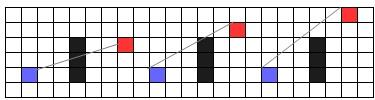
\includegraphics[width=\columnwidth]{./art/images/ffrpg-los.png}
\hspace*{1cm} No LoS \hspace*{0.8cm} LoS but no LoE \hspace*{0.5cm} LoS and LoE\\
\begin{center}
	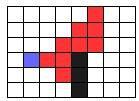
\includegraphics[width=0.4\columnwidth]{./art/images/ffrpg-obstacle.png}
\end{center}
\hfill Cone 4 against an obstacle \hfill
\ofrow
%
%\pagebreak\\
%
\ofaccent{Giant Characters:} Some characters may be greater than one square, occupying all of them at one time. 
For example, a monster may occupy a 2x2 square, a 3x3 square, a 2x1 rectangle or any other shape. 
When moving, giant characters treat all Difficult or Hazardous Terrain as Normal Terrain, unless all squares they occupy are Difficult or Hazardous. Deadly Terrain is treated as Hazardous Terrain for Giant Characters, unless all squares they occupy are Deadly.
Impassable Terrain is treated as Difficult Terrain unless it covers at least one side of the giant character (For example, a 2-square wide wall will block the movement from a 2x2 giant, but not a 3x3 one). A giant traversing Impassable Terrain like this will have to pay 2 points of MOVE per square traversed until none of its squares are over Impassable Terrain.
When determining Line of Sight and Line of Effect to or from giant characters, you may choose any of the character’s squares as the origin or target of the line.
Giant characters are only out of another character’s LoS if all of its squares are outside the LoS. All attacks and spells that can hit at least one square of the giant character hit it. 
Lastly, when determining the range of the giant character’s actions, you may use any of its squares as the origin square.
%
\\\\
%
\ofaccent{Job Adjustments:} Several jobs have to be adjusted to work with the map combat rules. 
You can find the list of adjustments and new specialties for each Job, Action and Spell below. 
All weapon attacks not listed below use your weapon’s range. 
All reactions not listed below can be used whenever you meet its trigger, regardless of range. 
When a Spell or Action lists two different damages, one for single target and other for group target, use the single-target damage when it has only one character in its area of effect, and the group-target damage when it has more than one character in its area of effect.
%
\\\\
%
%
\ofaccent{\large Adept} \ofrow
\textbf{!Snake Fang:} R:4 E:0\\
\textbf{!Hallowed Bolt:} R:4 E:0\\
\textbf{!Black Sky:} R:4 E:0\\
\textbf{!Shadow Blade:} R:0 E:2. You are immune to the effects.\\
\textbf{!Stasis Strike:} R:3 E:0\\
\textbf{!Demi Shock:} R:4 E:0\\
\textit{Mana Safe}: R:3 E:0	\\
\textit{Elemental Overload}: Increase the modified abilities to E:1. You are immune to the effects.	\\
\textbf{!Shellburst Stab:} R:5 E:0\\
\textbf{!Soul Eater:} R:5 E:2\\
\textbf{!Divine Retribution:} R:5 E:2\\
%
\\\\
%
\ofaccent{\large Archer} \ofrow
\textit{Warning Volley:} You can only deal the damage to enemies inside your weapon range.\\
\textbf{!Reflex Shot:} Use your weapon’s range.\\
\textbf{!Barrage:} Use the weapon’s range. Attacks random enemies inside weapon range.\\
%
\\\\
%
\ofaccent{\large Artist} \ofrow
\textbf{!Dance:} R1* E:0. 
Two dances are exceptions: Fatal Flamenco targets four random enemies inside R: Move, and Forbidden Dance targets all enemies inside R: 0 E: Half Move.\\
\textbf{!Song:} R:4 E:0. Five songs are exceptions: Requiem: R:0 E:2. Seraph Song: R:4 E: 2 (target only allies). Hero’s Ryme: R: 0 E: 0. Earth Blues and Nameless Song: R:4 E:1\\
\textbf{!Mimic:} All mimics use the same range and effect as the original action, except for Take Over, which is R: 4 E: 0\\
\textbf{!Throw:} R: 4 E: 0\\
\textbf{!Legend:} R: 6 E: 0. The target ally must be inside this range for you to react.\\
\textbf{!Hater:} R: 4 E:0\\
\textbf{!Do Over:} R: 6 E: 0. The target ally must be
inside this range for you to react.\\
\textbf{Dedicated Fans:} You must be adjacent to the ally who reacts. Before you react, you may use the !Move action, either by spending the round’s free !Move action or by using an regular action to do so.
%
\\\\
%
\ofaccent{\large Black Mage} \ofrow
\textit{Elemental Burst:} The secondary target must be inside the spell's Range.
%
\\\\
%
\ofaccent{\large Black Magic} \ofrow
\textbf{R: 4 E: 0:} Fire, Blizzard, Thunder, Blind, Petrify, Toad, Stone, Sleep, Zombie, Condemn, Death, Poison, Water, Dark, Rasp,
Osmose, Drain, Syphon, Pain and Hex.\\
\textbf{R: 4 E: 1:} Fira, Firaga, Blizzara, Blizzaga, Thundara, Thundaga, Waterga and Scourge.\\
\textbf{R: 0 E: 3. (You are immune to the effects):} Magnitude and Quake \\
\textbf{R: 5 E: 0:} Bio, Venom, Meltdown, Freeze, Overcharge and Break.\\
\textbf{R: 4 E: 2:} Storm and Scathe.\\
\textbf{R: 5 E: 2. (You are immune to the effects):} Ultima and Doomsday.\\
\textbf{R: 7 E: 0:} Flare.
%
\\\\
%
\ofaccent{\large Blue Magic} \ofrow
\textbf{R: 1* E: 0:} Goblin Punch and Red Feast.\\
\textbf{R: 4 E: 0:} Choco Ball, Death Force, Flash, Transfusion, Acid, Degenerator, Dragon Force, Death Claw and Rippler.\\
\textbf{R: 5 E: 0:} Self-Destruct, Hastebreak, 1000 Needles, Flame Thrower, Magic Hammer and Wall Change.\\
\textbf{R: 4 E: 1:} Matra Magic and Seed Cannon.\\
\textbf{R: 4 E: Burst 3:} Nightsong and Frog Song.\\
\textbf{R: 4 E: Cone 3:} Poison Gas and Stare.\\
\textbf{R: 0 E: Burst 5:} Aqua Rake and Electrocute.\\
\textbf{R: 6 E: 2:} Earth Shake, Grand Train and Supernova.\\
\textbf{R: 0 E: 2:} Force Field, White Wind and Mighty Guard.\\
\textbf{R: 0 E: 8:} Level 3 Confuse, Roulette, Level 2 Old, Level 4 Flare and Level 5 Death.\\
\textbf{R: 0 E: Cone 5:} Bad Breath, Magic Breath and Stone Breath.\\
\textbf{R: 6 E: 0:} Shadow Flare.
%
\\\\
%
\ofaccent{\large Calls} \ofrow
\textbf{R: 4 E: 1:} Asura, Fenrir, Ifrit, Lakshmi, Ramuh, Shiva and Valefor (Basic Call).\\
\textbf{R: 4 E: 0:} Chocobo (Increase to E: 1 when using the Fat Chocobo).\\
\textbf{R: 0 E: 4:} Valefor (Greater Call, Choose up to three allies inside the area. After gaining the Flight status, you and all targets may move a number of squares up to half of your Move stat. All movement done before your attacks with this action ignores Zone of Control, unless the enemy is also under the Flight status effect).\\
\textbf{R: 5 E: 1:} Atomos, Carbuncle, Catoblepas (Greater Call), Golem, Kirin (Greater Call), Madeen, Titan and Unicorn (Greater Call) Sraphim, Mist Dragon and Madiun.\\
\textbf{R: 5 E: 0:} Catoblepas (Basic Call), Kirin (Basic Call), Unicorn (Basic Call), Bomb (The additional !Summon damage is dealt to E: 1* centered on the Call target) and Mind Flayer.\\
\textbf{R: 0 E: 3:} Silph (Deals damage to one enemy and heals all allies inside the area).\\
\textbf{R: 5: E: 2 (Targets only enemies):} Alexander, Bahamut (Greater Call), Diabolos, Kujata, Leviathan, Odin (Greater Call) and Zodiac.\\
\textbf{R: 6 E: 0:} Cerberus (Basic Call).\\
\textbf{R: 4 E: 2:} Cerberus (Greater Call, Choose up to four targets inside the area) and Crusader (Basic Call).\\
\textbf{R: 6 E: 1:} Phoenix (Greater Call, Deals damage inside the area of effect. Raises one ally inside the range, but not necessarily inside the area of effect).\\
\textbf{R: 4 E: 3:} Crusader (Greater Call).\\
\textbf{R: 7 E: 0:} Ragnarok.
%
\\\\
%
\ofaccent{\large Druid} \ofrow
\textit{Curse:} R: 4 E: 0.\\
\textbf{!Lore:} R: 4 E: 0.\\
\textbf{!Tame:} R: 1* E: 0 for the action, R:4 E:0 if used as a reaction.\\
\textbf{!Air Wave:} R: 6: E: 0 to deal damage, R:4 E:2 to grant Float.\\
\textbf{!Earth Slash:} R: 0 E: Line 7\\
\textbf{!Intimidate:} R: 4 E: 0\\
\textbf{!Weak Point:} R: 3: E: 0\\
\textbf{!Quagmire:} R: 4 E: 2. Choose one target inside the area of effect. You may use a powerup to affect all targets inside the area, according to the action description.\\
\textbf{!Parley:} R: 4 E: 0. \\
\textbf{!Truce:} R: 5 E: 2.
%
\\\\
%
\ofaccent{\large Geomancy} \ofrow
\textbf{R: 5 E: 0:} Gusty Wind, Gust, Icicle, Waterfall, Bottomless Pit, Back Alley, Phantom, Flame Blast, Antlion and Cosmic Flare.\\
\textbf{R: 1 E: 2 (Choose one target inside the area of effect. You may use a powerup to affect all targets inside the area, according to the Geomancy description.):}
Sunbath, Wild Bear, Crowd Cheer, Earth Shield, Shining Air, Cosmic Embrace and Great Convergence.\\
\textbf{R: 6 E: 2:} Pitfall and Plasma.\\
\textbf{R: 0 E: Burst 4:} Corrupt Water.\\
\textbf{R: 0 E: Cone 4:} Sandstorm.\\
\textbf{R: 4 E: 1:} Leaf Swirl.\\
\textbf{R: 6 E: 3:} Branch Spears (Targets random enemies inside the area).\\
\textbf{R: 5 E: 1:} El Niño, Cave In and Magma.\\
\textbf{R: 0 E: Burst 3:} Poison Mists and Desert Storm.\\
\textbf{R: 0 E: Cone 3:} Sonic Boom.\\
\textbf{R: 5 E: Line 4:} Landslide and Avalanche.\\
\textbf{R: 3 E: 0:} Ice Armor.\\
%
\\\\
%
\ofaccent{\large Monk} \ofrow
\textbf{!Doton:} R: 3 E: 0. Change to R: 0 E: Burst 3 with the Elan Specialty.\\
\textbf{!Fuuton:} R: 3 E: 0. Change to R: 3 E: 1 with the Elan Specialty.\\
\textbf{!Katon:} R: 3 E: 0. Change to R: 0 E: Line 5 with the Elan Specialty.\\
\textbf{!Suiton:} R: 3 E: 0. Change to R: 0 E: Cone 3 with the Elan Specialty.\\
\textbf{!Raiton:} R: 0 E:0 when used to defend yourself, or R: 3 E: 0 to defend an ally.\\
\textbf{!Kick:} R: 2 E: 1*\\
\textbf{!Aura Bolt:} R: 5 E: 0\\
\textbf{!Dark Bolt:} R: 5 E: 0\\
\textbf{!Atemi:} R:1* E:0\\
\textbf{!Chi Blast:} R:1* E:0\\
\textbf{!Kuuton:} R:4 E:2\\
\textbf{!Phantom Rush:} R:1* E:0
%
\\\\
%
\ofaccent{\large Rogue} \ofrow
\textbf{!Steal:} R: 1* E: 0\\
\textbf{!Detect:} R: 4 E: 0\\
\textbf{!Peep:} R: 4 E: 0\\
\textbf{!Lucky Odds:} R: 4 E: 0\\
\textbf{!Karma:} R: 6 E: 0. The target enemy must be inside this range for you to react.\\
\textbf{!Dice:} R: 3 E: 0\\
\textbf{!Dismantle:} R:1* E:0\\
\textbf{!Moogle Reels:} R:4 E:1. Targets only enemies.\\
\textbf{!Lucky Seven:} R: 6 E: 0. The target enemy must be inside this range for you to react.\\
\textbf{!Gil Toss:} R: 0 E: 3. Targets all enemies in the area.\\
\textbf{!Chocobo Reels:} R:4 E:2. You may choose between targeting only enemies or only allies.\\
\textbf{!Steal Heart:} R: 4 E: 0\\
\textbf{!Distract:} R: 1* E: 0
%
\\\\
%
\ofaccent{\large Time Mage} \ofrow
\textbf{!Phase:} After being successful, choose a square adjacent to the attack’s area of effect. You teleport to that square.\\
\textbf{!Delay:} R: 6 E: 0. The character using the spell must be inside this range for you to react.
%
\\\\
%
\ofaccent{\large Time Magic} \ofrow
\textbf{R: 4 E: 0:} Burn Ray, Remove, Gravity, Demi, Quarter, Black Hole, Yawn, Slow, Stop, Mental Down, Armor Down, Power Down, Magic Down, Mental Up, Armor Up, Power Up, Magic Up, Speed Up, Tractor, Flight, Haste, Regen, Immobilize, Disable and Reset.\\
\textbf{R: 0 E: 0:} Escape (You teleport to an adjacent square. For each 5 levels in Fire, you can teleport one extra square. You still have to be successful to leave Zone of Control) and Quicken.\\
\textbf{R: 0 E: 3:} You and your allies teleport to an adjacent square. For each 2 levels in Fire, you can teleport one extra square. You still have to be successful to leave Zone of Control.\\
\textbf{R: 4 E: 1:} Ray Bomb, Quasar, Shockwave Pulsar, X-Zone, Slowga, Hastega, Float and Return.\\
\textbf{R: 4 E: 2 (Targets random enemies inside the area):} Meteorite, Comet and Meteo.\\
\textbf{R: 6 E: 0:} Old.\\
\textbf{R: 6 E: 1:} Time Stop.\\
\textbf{R: 5 E: 3 (Targets random enemies inside the area):} Meteor.
%
\\\\
%
\ofaccent{\large Warrior} \ofrow
\textbf{!Arc:} R:4 E:0\\
\textbf{!Jump:} After gaining the Flight status, you may move a number of squares up to half your Move stat. All movement done before you attack with this action ignores Zone of Control, unless the enemy is also under the Flight status effect.\\
\textbf{!Minus Strike:} R:1* E:0\\
\textbf{!Dirty Fighting:} R:1* E:0\\
\textbf{!Pommel Strike:} R:1* E:0\\
\textbf{!Quadra Slam:} R:0 E:3. Targets four random enemies inside the effect area.\\
\textbf{!Guardbreak:} R:1* E:0\\
\textbf{!Armor Break:} R:1* E:0. You may change it to Burst 2 with the Mastery of Destruction Specialty.\\
\textbf{!Magic Break:} R:1* E:0. You may change it to Burst 2 with the Mastery of Destruction Specialty.\\
\textbf{!Mental Break:} R:1* E:0. You may change it to Burst 2 with the Mastery of Destruction Specialty.\\
\textbf{!Power Break:} R:1* E:0. You may change it to Burst 2 with the Mastery of Destruction Specialty.\\
\textbf{!Slash All:} R: 0 E: Burst 3.\\
\textbf{!Blade Beam:} R: 5 E: Cone 3. The primary target is the cone origin square. Targets secondary targets inside the cone area.\\
\textbf{!Dragon Breath:} R:1* E:0\\
\textbf{!Shock:} R: 0 E: 3. You are immune to the effects.\\
\textbf{!Cleave:} R: 4 E: 2. You are immune to the effects.
%
\\\\
%
\ofaccent{\large White Magic} \ofrow
\textbf{R: 4 E: 0:} Cure, Poisona, Basuna, Esuna, Aero, Banish, Resist, Immune, Absorb, Raise, Arise, Reraise, Protect, Wall, Shell, Reflect, Blink, Vanish, Silence, Berserk, Confuse, Charm, Scan, Weaken and Shield.\\
\textbf{R: 4 E: 1:} Cura, Curaga, Aera, Aeraga, Banishra, Banishga, Protectga, Shellga, Ruse, Vaccine and Rebirth.\\
\textbf{R: 5 E: 0:} Fade and Renew.\\
\textbf{R: 4 E: 1:} Whirlwind.\\
\textbf{R: 6 E: 0:} Holy.
%
%
\pagebreak\\
%
%
\ofaccent{\large Alchemist} \ofrow
\textbf{!Treatment:} R: 4 E: 0\\
\textbf{Distribute:} R:0 E: 2. The area is centered on the character healed. Targets only allies.\\
\textbf{!Mix:} Healing items that target a Group with !Mix heal on an E: 1 area.\\
\textbf{New Quick Hands Specialty:} Throw Item: Requires Air level 4. When you use healing items, they reach R: 4 instead of R: 1*.\\
\textbf{New Quick Hands Specialty:} Battlefront Medic: Requires Air and Earth level 3. Once per round, when you use the \textbf{!Draw} action, you may use the \textbf{!Move} action as a free action.\\
\textbf{Pharmacology Specialty:} Versatile Apotechary: Requires Earth level 10. Choose and gain one \textit{Quick Hands Specialty}.
%
\\\\
%
\ofaccent{\large Berserker} \ofrow
\textbf{Counter Attack:} Before you Counter Attack, you may use the \textbf{!Move} action, either by spending the round’s free \textbf{!Move} action or by using an regular action to do so.\\
\textbf{!Hamedo:} Has the same range as your \textbf{!Attack} action.\\
\textbf{!Provoke:} R: 4 E: 0\\
\textbf{!Howl:} R: 4 E: 0\\
\textbf{Dispel:} R: 5 E: 0\\
\textbf{New Counter Attack Specialty:} Nimble Retort: Requires Water level 3. When you declare your Counter Attack, ignore enemy Zone of Control this phase.\\
\textbf{New Provoke Specialty:} Counter Disengage: Requires Water level 9. You can Counter Attack when enemies declare the \textbf{!Escape} action against you.\\
\textbf{New Fury Specialty:} Stand Ground: Requires Fire level 13. While you wield a Melee weapon and has not used \textbf{!Move} this round, your Counter Attacks are free actions.
%
\\\\
%
\ofaccent{\large Defender} \ofrow
\textbf{!Cover:} To use \textbf{!Cover}, you must be adjacent to either the attacker or the ally who was hit or either one must be inside your Zone of Control.\\
\textbf{Sentinel:} Before you react, you may use the \textbf{!Move} action, either by spending the round’s free \textbf{!Move} action or by using an regular action to do so.\\
\textbf{Healing Wind:} Your Healing group Spells are all R: 4 E: 1.\\
\textbf{!Shared Pain:} R: 1* E: 0.\\
\textbf{Noble Sacrifice:} To use it, you must be adjacent to either the attacker or the ally who was hit or either one must be inside your Zone of Control.\\
\textbf{Astra:} R: 4 E: 0\\
\textbf{Perseus’ Mirror:} The mirrored attack retains its original R and E values, using the Defender as the origin point of the range.\\
\textbf{Astraga:} R: 5 E: 2\\
\textbf{Great Gospel:} R: 0 E: 0\\
\textbf{New Cover Specialty:} Trip: Requires Earth level 4. Whenever an enemy try to use the \textbf{!Flee} action against you, use the greater between Air or Earth as the Defensive Stat.\\
\textbf{New Cover Specialty:} Mobile Defense: Requires Air level 4. You may treat your Zone of Control as being R: 3 to use other abilities.\\
\textbf{New Share the Pain Specialty:} Vanguard: Requires Air and Water level 7. Allied characters ignore enemy Zone of Control while moving inside your Zone of Control.
%
\\\\
%
\ofaccent{\large Dervish} \ofrow
\textbf{New Ambidexterity Specialty:} Combat Dash: Requires Fire level 3. Each round, you may use a \textbf{!Move} action at the start of the first phase, either by spending the round’s free \textbf{!Move} action or by using an regular action to do so.\\ 
\textbf{New Ambidexterity Specialty:} Bladedancer: Requires Air and Water level 4. Whenever you use the \textbf{!Attack} action, you may move one square before attacking. This movement ignores Zone of Control.\\ 
\textbf{New Critical Speed Specialty:} Guardbreaker: Requires Earth and Air level 7. Enemies hit by your weapon do not project Zone of Control this phase.
%
\\\\
%
\ofaccent{\large Fencer} \ofrow
\textbf{!Bobbing:} R: 5 E: 0.\\
\textbf{New Block Projectiles Specialty:} Elusive Movement: Requires Air level 5. When you declare the \textbf{!Move} action, choose one enemy. You ignore that enemy’s Zone of Control.\\
\textbf{New Preemptive Strike Specialty:} Indirect Shot: Requires Earth level 12. Increase the range of your Ranged physical attacks by one square.\\
\textbf{New Preemptive Strike Specialty:} Earth Dancer: Requires Earth level 8. Whenever an an opponent misses an attack against you or you avoid its affects by reacting, you may move one square. Increase this movement to two squares at level 50. This movement ignores Zone of Control.
%
\\\\
%
\ofaccent{\large Phalanx} \ofrow
\textbf{Huge Target} Only effects enemies inside R: 5.\\
\textbf{!Testudo:} To use \textbf{!Testudo}, you must be adjacent to either the attacker or the ally who was hit or either one must be inside your Zone of Control.\\
\textbf{!Shield Wall:} To use \textbf{!Shield Wall}, you must be adjacent to either the attacker or the ally who was hit or either one must be inside your Zone of Control.\\
\textbf{Unshakable} The first option only effects enemies inside your weapon range.\\
\textbf{!Meatbone Slash:} R: 1 E: 0\\
\textbf{New Impenetrable Specialty:} Defensive Formation: Requires Air level 3. Whenever an enemy performs an attack that does not target you, you may move one square.\\
\textbf{New Tireless Specialty:} Hold the Front: Requires Air level 11. Your Zone of Control is Difficult Terrain for enemies.\\
\textbf{New Unshakable Specialty:} Towering Shield: Requires Earth and Air level 11. Whenever you are hit by a physical attack, treat your square as Impassable Terrain to determine LoS and LoE until the end of this round.
%
\\\\
%
\ofaccent{\large Rune Knight} \ofrow
\textbf{Runic Area:} To use \textbf{!Runic} to protect an ally, you must be adjacent to either the attacker or the ally who was hit or either one must be inside your Zone of Control.\\
\textbf{Offensive Runes:} Your \textbf{!Runic} becomes R: 6 E: 0. The target of the spell must be inside that range.\\
\textbf{!Magic Ruin:} R: 4 E: 0\\
\textbf{!Dispel Strike:} As your weapon’s range.\\
\textbf{Anti-Magic Zone:} Your \textbf{!Dispel Strike} becomes R: 0 E: 4\\
\textbf{!Triple Magic:} As the original Spell.\\
\textbf{!Spell Ruin:} R: 1 E: 0\\
\textbf{New Spell Protection Specialty:} Mage Hunter: Requires Air level 3. Whenever an enemy casts a Spell, you may use the \textbf{!Move} action as an interrupt, ignoring all Zone of Control except the spellcaster's.\\
\textbf{New Spell Protection Specialty:} Arcane Weapons: Requires Fire and Water level 5. Your Instruments and Wands weapons project Zone of Control as if they were Melee.\\
\textbf{New Dispel Magic Specialty:} Spellshield: Requires Fire and Water level 11. Whenever you are hit by a Spell or magical attack, treat your square as Impassable Terrain to determine LoS and LoE until the end of this round.
%
\\\\
%
\ofaccent{\large Squire} \ofrow 
\textbf{!Throw Stone:} R: 4 E: 0\\
\textbf{!Awareness:} R: 0 E: 5\\
\textbf{!Yell:} R: 4 E: 0\\
\textbf{Ordered Retreat:} All allies may move as if they had used the \textbf{!Flee} action.\\
\textbf{New Basic Skill Specialty:} Dash: Requires Earth 3. You gain the Melee Quick physical action \textbf{!Dash}. You bodyslam at your target, attacking with your weapon. Do a weapon attack, inflicting normal damage, and pushing your target one square backwards. If you manage to achieve a critical hit, the target is also gains the \textbf{Immobilize} status until after his next action. R: 1* E: 0\\
\textbf{New Basic Skill Specialty:} Move-Up: Requires Air 3. Increase your MOVE by 1.\\
\textbf{New Accumulate Specialty:} Magical Traps: Requires Fire and Earth 11. You may create magical traps. When using a magical ability or Spell, you may target a square in range and any phase up to the end of the next round. At the start of the chosen phase, the Ability or Spell detonates, inflicting its effects, and using the chosen square as the origin point of the Area of Effect, if applicable. Whenever a character moves into the chosen square before the chosen phase, you may detonate the trap early.
%
\\\\
%
\ofaccent{\large Wizard} \ofrow 
\textbf{!Counter Magic:} When used as a Sage, the original caster must be inside your spell's range.\\
\textbf{!Shieldbreak:} R: 0 E: 2\\
\textbf{New Counter Magic Specialty:} Distant Spell: Requires Fire level 12. Your Spells with R: 2 or greater increase their range by one square.\\
\textbf{New Counter Magic Specialty:} Contagion: Requires Earth and Air level 12. Your Spells with E: 1 or greater may also hit one extra target adjacent to the area of effect.\\
\textbf{New Silent Spell Specialty:} Graceful Casting: Requires Earth and Water level 14. As a \textit{Sage}, whenever you cast a Spell, you may choose up to two characters in the Spell's area of effect. Your spell does not target the chosen characters. As a \textit{Red Mage}, whenever you cast a Spell with E: 1, you may choose to cast it as a R:0 Cone 3 or Burst 3 instead, and whenever you cast a Spell with E: 2, you may choose to cast it as a R:0 Cone 4 or Burst 4 instead.
%
\\\\
%
%
\\\\
%
%
\ofaccent{\large Ivalice Bestiary} \ofrow 
%
Most of the enemies in the game are regular human beings, but there are several monsters in Ivalice. Below are some examples, but be sure to check for more monsters in the game's \href{http://ffrpg4e.wikidot.com/bestiary/}{wiki bestiary}.
%
\vfill
%
\ffrpgmonster{Floating Eye}{10}{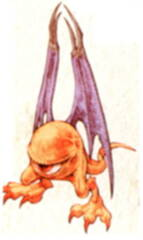
\includegraphics[width=0.21\textwidth]{./art/monsters/eye.jpg}}
{Beast Aberration \hfill Minion}
{
	Earth: & \hfill 12   & Air:   & \hfill 41\\
	Fire:  & \hfill 38   & Water: & \hfill 24\\
	HP:    & \hfill 49   & MP:    & \hfill 20\\
	ARM:   & \hfill 2    & MARM:  & \hfill 10\\
	Move:  & \hfill 5    & Init:  & \hfill 2d\\
}
{Vulnerable (Ice), Resist (Air), Vulnerable (Blind), \\Auto-Flight}
{
	\ofaccent{Wing Buffet:} Quick physical action, Air vs Earth, diff 40, 24 damage (Crush) and move the target 1 square, R1* E0\ofrow
	\ofaccent{Dread Gaze:} Ranged Slow (2) magical Action, Fire vs Fire, diff 40, inflicts \textbf{Weaken (Physical)} until end of next turn, R4 E0\ofrow
	\emph{Huge eyeballs with wings, these aberrations travel in flocks and use a baleful stare to attack their enemies. The strongest forms of these enemies can even petrify their foes with just a glare.}
}
%
\clearpage
\onecolumn
\begin{multicols}{2}
%
\ffrpgmonster{Grenade}{20}{
\includegraphics[width=0.28\textwidth]{./art/monsters/bomb.jpg}}
{Elem. Aberration \hfill Common}
{
	Earth: & \hfill 34   & Air:   & \hfill 54\\
	Fire:  & \hfill 72   & Water: & \hfill 58\\
	HP:    & \hfill 249  & MP:    & \hfill 120\\
	ARM:   & \hfill 12   & MARM:  & \hfill 14\\
	Move:  & \hfill 4    & Init:  & \hfill 3d\\
}
{Vulnerable (Ice and Water), Immune (Fire), \\Auto-Float}
{
	\ofaccent{Tackle:} Quick physical action, Air vs Earth, diff 40, 25 damage (Crush), R1* E0\ofrow
	\ofaccent{Fire:} Black Spell, 8 MP, Fire vs Water, diff 0, 35 damage (Fire), R4 E0\ofrow
	\ofaccent{Oil:} Spell, 42 MP, Fire vs Water, diff 70, inflicts \textbf{Fire Vulnerable} until the end of next round, R5 E0\ofrow
	\ofaccent{Self-Destruct:} Blue Spell, 1 MP, Fire vs Water, diff 0, kill it self to do damage equal to HP (non-elemental), R5 E0\ofrow
	\emph{The result of a failed magical experiment, these ravenous creatures hunt places imbued with magic. Some unethical mages still hope to devise a way to control them.}
}
%
\\\\
%
\ffrpgmonster{Goblin}{27}{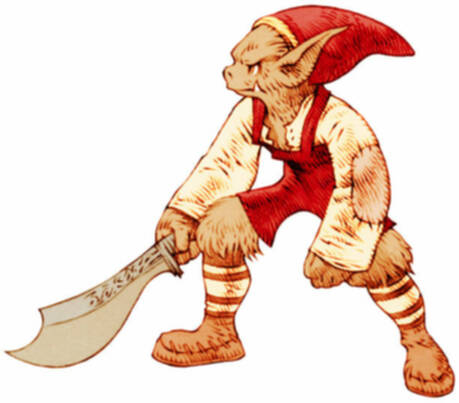
\includegraphics[width=0.34\textwidth]{./art/monsters/goblin.jpg}}
{Humanoid Undead \hfill Common}
{
	Earth: & \hfill 91   & Air:   & \hfill 87\\
	Fire:  & \hfill 46   & Water: & \hfill 60\\
	HP:    & \hfill 250  & MP:    & \hfill 40\\
	ARM:   & \hfill 22   & MARM:  & \hfill 18\\
	Move:  & \hfill 5    & Init:  & \hfill 3d\\
}
{Vulnerable (Ice and Shadow)}
{
	\ofaccent{Tackle:} Quick physical action, Earth vs Air, diff 40, 45 damage (Cut), R1* E0\ofrow
	\ofaccent{Spin Punch:} Quick physical action, Air vs Air, diff 40, 40 damage (Crush), attacks all enemies, R0 E1*\ofrow
	\ofaccent{Eye Gouge:} Quick physical action, Air vs Earth, diff 70, 40 damage (Puncture), inflicts \textbf{Blind} and reduce MOVE by 1 until the end of next turn, R1* E0\ofrow
	\emph{Diminute humanoids with limited speech, these tribal foes have large ears and an upturned nose. Surprisingly strong for its small size.}
}
%
\columnbreak\\
%
\ffrpgmonster{Red Chocobo}{30}{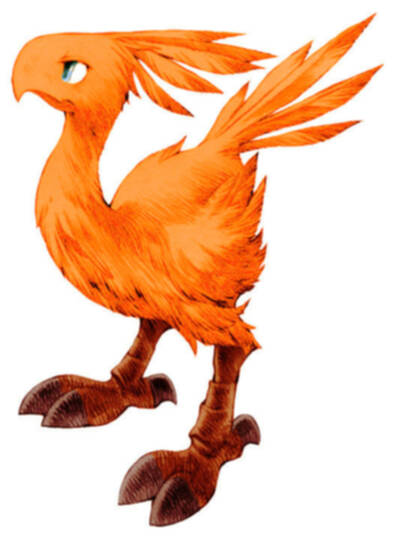
\includegraphics[width=0.25\textwidth]{./art/monsters/chocobo-red.jpg}}
{Beast \hfill Minion}
{
	Earth: & \hfill 61   & Air:   & \hfill 92\\
	Fire:  & \hfill 80   & Water: & \hfill 76\\
	HP:    & \hfill 255  & MP:    & \hfill 256\\
	ARM:   & \hfill 42   & MARM:  & \hfill 37\\
	Move:  & \hfill 6    & Init:  & \hfill 2d\\
}
{Vulnerable (Air and Earth), Immune (Curse)}
{
	\ofaccent{Beak:} Quick physical action, Air vs Air, diff 40, 54 damage (Puncture), R1* E0\ofrow
	\ofaccent{Choco Dodge:} Reaction, Air vs Air, dif 40, avoids a physical attack, R0 E0\ofrow
	\ofaccent{Choco Mobility:} Each time it uses the \textbf{!Move} action, the Red Chocobo may ignore one enemy's Zone of Control\ofrow
	\ofaccent{Choco Meteor:} Spell, 64 MP, Fire vs Water, diff 0, 64 damage (Crush). Push each target hit not on the central square of the effect one square away from the central square of the effect, R4 E1.\ofrow
	\emph{It is said those feral chocobos are descendants of a legendary chocobo breeder in the Ronan Empire. Their bottled anger comes from knowing they'll never go back home.}
}
%
\\\\
%
\ffrpgmonster{Revenant}{39}{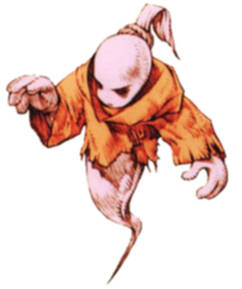
\includegraphics[width=0.28\textwidth]{./art/monsters/ghost.jpg}}
{Humanoid Undead \hfill Common}
{
	Earth: & \hfill 92   & Air:   & \hfill 94\\
	Fire:  & \hfill 128  & Water: & \hfill 94\\
	HP:    & \hfill 608  & MP:    & \hfill 502\\
	ARM:   & \hfill 46   & MARM:  & \hfill 69\\
	Move:  & \hfill 4    & Init:  & \hfill 3d\\
}
{Vulnerable (Light and Fire), Resist (Ice), Absorb (Shadow), Immune (Transform, Toxic, Mental), Auto-Float, Auto-Zombie}
{
	\ofaccent{Ectoplasm:} Ranged Quick magical action, Fire vs Earth, dif 40, 120 damage (Shadow), R3 E0\ofrow
	\ofaccent{Sleep Touch:} Slow (2) magical action, Fire vs Water, dif 60, inflicts \textbf{Sleep} until end of next turn, R1* E0\ofrow
	\ofaccent{Weaken:} White Spell, 82 MP, Fire vs Water, dif 70, inflicts \textbf{Vulnerability(chosen element)} until end of next turn, R4 E0\ofrow
	\ofaccent{Roulette:} Blue Spell, 80 MP, Fire vs Water, dif 40, inflict \textbf{Death} to a random target, R0 E8\ofrow
	\emph{A restless incorporeal spirit. A mere touch may suck the life from its target, causing debilitating status effects. These are amongst the strongest of the ghosts found in the old ruins and wastelands of Ivalice.}
}
%
%
\end{multicols}
%
\vfill
\begin{center}\ofquote{"The moment pride is lost, freedom is also lost."}{Ramza Belouve}\end{center}
%
\twocolumn
\clearpage